\section{\centering Численные эксперименты}
\subsection{\centering Проверка стабильности имитационной модели}
Для начала проведения численного анализа полученных асимптотических результатов необходимо проверить точность работы реализованной имитационной модели. Для проверки, запустим модель несколько раз с одинаковыми параметрами и для полученных результатов вычислим критерий согласия Колмогорова. Критерий согласия Колмогорова (расстояние Колмогорова) предназначен для проверки гипотезы о том, что некое эмпирическое распределение, в данном случае, распределение, построенное в ходе работы имитационной модели, соответствует предполагаемой модели, которая, в данном случае, так же является результатом работы имитационной модели.

Расстояние Колмогорова вычисляется по следующей формуле
\begin{equation*}
	\Delta_{l} = \underset{0 \leq i \leq \infty}{max}\bigg\rvert \sum_{v=0}^{i} (P(v) - P^{l}(v))\bigg\rvert, l = 1,2
\end{equation*}
Для численного анализа в данной работе применяется система компьютерной алгебры Mathcad. В ней были построены графики распределения вероятностей и вычислено расстояния Колмогорова для двух запусков имитационной модели с одинаковыми параметрами системы

\begin{figure}[H]
	\centering
	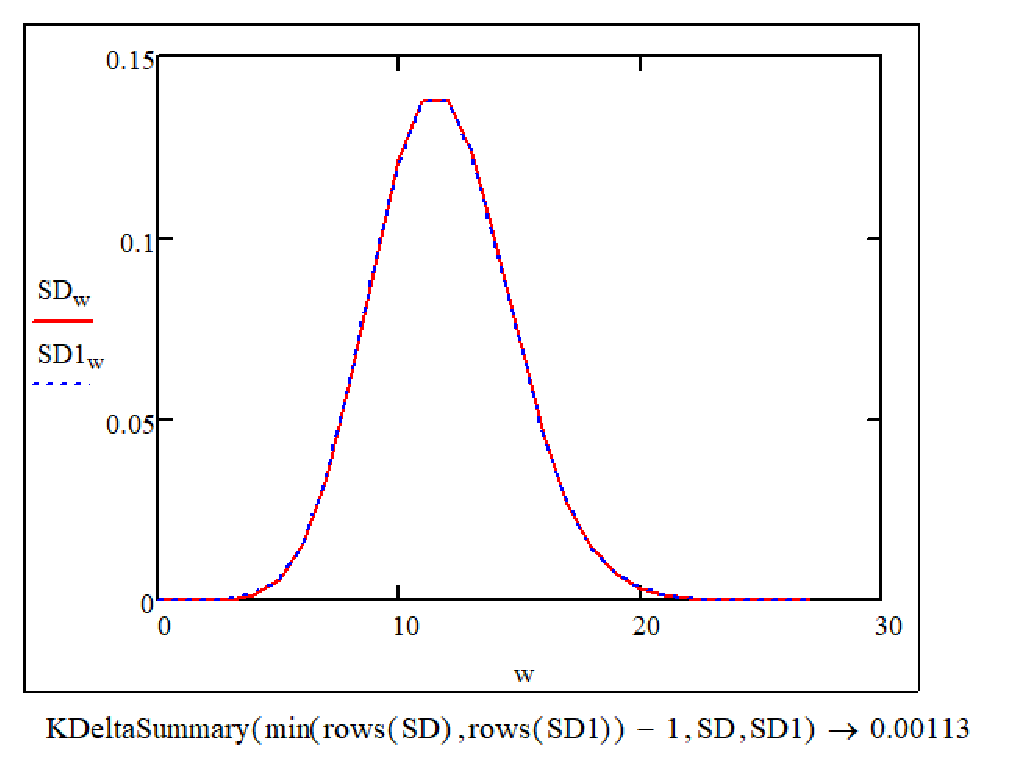
\includegraphics[scale=0.5,width=\textwidth]{mathcad_check_sim.eps}
	\caption{Сравнение двух отдельных запусков имитационной модели с простейшим входящим потоком}
	\label{experiments_kol_dist_sim}
\end{figure} 

На рисунке \ref{experiments_kol_dist_sim} представлено сравнение двух запусков имитационной модели с параметрами системы: $\lambda = 1, \alpha = 0.5, \sigma = 0.4, \mu_{1} = 6, \mu_{2}, t = 10 $. Запуски модели дали практически одинаковые результаты. Вычисленное расстояние Колмогорова составило  0.000596 для суммарного распределения и 0.0016632 для двумерного распределения. Графики плотности распределения вероятностей полностью накладываются друг на друга.

\begin{figure}[H]
	\centering
	\includegraphics[scale=0.5,width=\textwidth]{mathcad_check_sim2.eps}
	\caption{Сравнение двух отдельных запусков имитационной модели с MMPP--потоком}
	\label{experiments_kol_dist_sim2}
\end{figure} 

Данный эксперимент был проведен и для системы с входящим MMPP--потоком. Были заданы следующие параметры: $\alpha = 0.5, \sigma = 0.4, \mu_{1} = 6, \mu_{2}, t = 10 $,
\begin{equation*}
	\boldsymbol{Q}=\begin{bmatrix}
		-0.3 &  0.1 &  0.2\\
		0.2 & -0.5 &  0.3\\
		0.3 &  0.3 &  -0.6
	\end{bmatrix}
\end{equation*}

\begin{equation*}
	\boldsymbol{\Lambda}=\begin{bmatrix}
		1 &	0 & 0\\
		0 &	0.6 & 0\\
		0 &	0 & 0.7\\
	\end{bmatrix}.
\end{equation*}
Результаты эксперимента представлены на рисунке \ref{experiments_kol_dist_sim2}. Для суммарного распределения расстояние Колмогорова составило 0.00059, для двумерного --- 0.001258. Графики плотности распределений также полностью накладываются друг на друга.

Исходя из вышеописанных экспериментов, можно сделать вывод, что реализованная имитационная модель дает стабильные результаты, что подтверждают вычисленные значения расстояния Колмогорова для обоих видов распределений --- его значение не превышает порог в 0.002. Следовательно, модель может быть применена для анализа и оценки применимости асимптотических результатов.
\subsection{\centering Сравнение распределений вероятностей с эмпирическим распределением}
Теперь, когда стабильность имитационной модели подтверждена экспериментально, сравним результаты ее работы с полученным асимптотическим приближением функции распределения вероятностей числа обслуженных заявок для систем, рассмотренных в разделах \ref{section_simple_summary}, \ref{section_simple_twodim} и \ref{section_map_twodim} при разной интенсивности возврата заявок с орбиты. Значение этого параметра влияет на точность при сравнении, так как решение систем было получено при асимптотическом условии большой задержки заявок на орбите.

Для того, чтобы проиллюстрировать влияние задержки заявок на орбите на получаемый результат для RQ--системы с простейшим входящим потоком, зададим ее параметры:
\begin{equation} \label{simple_summary_input_params}
	\lambda = 2,
	\alpha = 0.9,
	\mu_{1} = 3.5,
	\mu_{2} = 2.1, 
	t = 15
\end{equation}
Теперь, рассчитаем распределения вероятностей числа обслуженных заявок по формуле \eqref{distr_simple_summary} и сделаем несколько запусков имитационной модели, варьируя интенсивность возращения заявок с орбиты $\sigma$.

Введем следующие обозначения: $\Delta_S$ --- расстояние Колмогорова для суммарного распределения вероятностей, $\Delta_{TD}$ --- расстояние Колмогорова для двумерного распределения

\begin{table}[h!] 
	\centering
	\caption{Расстояние Колмогорова при различных значениях параметра $\sigma$}
	\label{table_simple_summary}
	\begin{tabular}{| c | c | c | c | c | c | c | c | c |}
		\hline
		$\sigma$ & 10 & 1 & 0.6 & 0.4 & 0.2 & 0.1 & 0.05 & 0.01 \\ 
		\hline
		$\Delta_S$ & 0.0216 & 0.0148 & 0.0112 & 0.0096 & 0.0062 & 0.0044 & 0.0023 & 0.0019\\
		\hline
		$\Delta_{TD}$ & 0.0398 & 0.02619 & 0.0205 & 0.0153 & 0.0088 & 0.0056 & 0.0025 & 0.0019\\
		\hline
	\end{tabular}
\end{table}

Как видно в таблице \ref{table_simple_summary}, при сравнении работы имитационной модели и асимптотических результатов расстояние Колмогорова тем меньше, чем меньше интенсивность возврата заявок с орбиты. Однако, даже при больших значениях $\sigma$, таких как 10 и 1, мы получаем результаты, где расстояние Колмогорова составляет не больше четырех сотых. В нижней строчке таблицы \ref{table_simple_summary} представлены расчеты для двумерного распределения вероятности числа обслуженных заявок. Можно видеть, что в случае двумерного распределения расстояние Колмогорова значительно больше при больших значениях $\sigma$, однако оно сходится к такому же значению при $\sigma = 0.01$, что и в случае одномерного распределения.

Чтобы проверить, наблюдается ли подобная тенденция при большей загруженности системы, установим в ранее описанных параметрах \eqref{simple_summary_input_params} $\lambda = 2.7$. Тогда получим следующий результат

\begin{table}[h!] 
	\centering
	\caption{Расстояние Колмогорова при различных значениях параметра $\sigma$ при повышенной интенсивности прихода заявок}
	\label{table_simple_summary_high_lambda}
	\begin{tabular}{| c | c | c | c | c | c | c | c | c |}
		\hline
		$\sigma$ & 10 & 1 & 0.6 & 0.4 & 0.2 & 0.1 & 0.05 & 0.01 \\ 
		\hline
		$\Delta_S$ & 0.0068 & 0.0044 & 0.0039 & 0.0028 & 0.003 & 0.0025 & 0.0013 & 0.0016\\
		\hline
		$\Delta_{TD}$ & 0.021 & 0.0104 & 0.0074 & 0.0044 & 0.0034 & 0.0021 & 0.0017 & 0.0011\\
		\hline
	\end{tabular}
\end{table}

Как видно в таблице \ref{table_simple_summary_high_lambda}  при повышенной загруженности системы также наблюдается тенденция к уменьшению расстоянию Колмогорова, однако, асимптотические результаты оказываются значительно точнее.

Поскольку интенсивность вызова прибором заявок также влияет на количество заявок на орбите, проведем расчеты с параметрами \eqref{simple_summary_input_params}, установив $\alpha = 1.6$

\begin{table}[h!] 
	\centering
	\caption{Расстояние Колмогорова при различных значениях параметра $\sigma$ при повышенной интенсивности вызова заявок}
	\label{table_simple_summary_high_alpha}
	\begin{tabular}{| c | c | c | c | c | c | c | c | c |}
		\hline
		$\sigma$ & 10 & 1 & 0.6 & 0.4 & 0.2 & 0.1 & 0.05 & 0.01 \\ 
		\hline
		$\Delta_S$ & 0.007 & 0.0062 & 0.0051 & 0.0054 & 0.0053 & 0.0023 & 0.0013 & 0.002\\
		\hline
		$\Delta_{TD}$ & 0.0242 & 0.015 & 0.0111 & 0.0096 & 0.0069 & 0.0029 & 0.0015 & 0.0011\\
		\hline
	\end{tabular}
\end{table}

Из расчетов в таблице \ref{table_simple_summary_high_alpha} видно, что также при увеличении задержки заявок на орбите, асимптотические результаты становятся точнее, однако повышение интенсивности вызова прибором заявок делает расчеты менее закономерными.

Для проведения данного эксперимента с RQ--системой, где в качестве источника заявок выступает MMPP--поток, зададим следующие параметры:
\begin{equation*} \label{map_summary_input_params}
	\alpha = 0.6,
	\mu_{1} = 2,
	\mu_{2} = 1.5, 
	t = 15,
\end{equation*}
 \begin{equation*}
 	\boldsymbol{Q}=\begin{bmatrix}
 		-0.5 &  0.2 &  0.3\\
 		0.15 & -0.2 &  0.05\\
 		0.3 &  0.4 &  -0.7
 	\end{bmatrix},
 \end{equation*}
 
 \begin{equation*}
 	\boldsymbol{\Lambda}=\begin{bmatrix}
 		1 &	0 & 0\\
 		0 &	0.6 & 0\\
 		0 &	0 & 0.7\\
 	\end{bmatrix}.
 \end{equation*}
\\
Для них были получены следующие результаты
\begin{table}[h!] 
	\centering
	\caption{Расстояние Колмогорова при различных значениях параметра $\sigma$ при моделировании MMPP-потока}
	\label{table_map_summary}
	\begin{tabular}{| c | c | c | c | c | c | c | c | c |}
		\hline
		$\sigma$ & 10 & 1 & 0.6 & 0.4 & 0.2 & 0.1 & 0.05 & 0.01 \\ 
		\hline
		$\Delta_S$ & 0.05312 & 0.045 & 0.0407 & 0.0359 & 0.0282 & 0.023 & 0.018 & 0.0163\\
		\hline
		$\Delta_{TD}$ & 0.0587 & 0.0493 & 0.0415 & 0.0348 & 0.0236 & 0.0154 & 0.009 & 0.0028\\
		\hline
	\end{tabular}
\end{table}

Ввиду того, что MMPP--поток труднее поддается моделированию, расстояние Колмогорова для расчетов с ним в среднем больше, однако при маленьких значениях $\sigma$ точность значительно увеличивается. Также, на таблице \ref{table_map_summary} можно заметить, что при меньших $\sigma$ для двумерного распределения асимптотические результаты оказываются точнее.

Повысим загруженность системы, задав новую матрицу интенсивностей с более высокими значениями диагональных элементов 
 \begin{equation*}
	\boldsymbol{\Lambda}=\begin{bmatrix}
		1.2 &	0 & 0\\
		0 &	0.9 & 0\\
		0 &	0 & 1.5\\
	\end{bmatrix}.
\end{equation*}

Проведем эксперимент с новыми параметрами и получим

\begin{table}[htb!] 
	\centering
	\caption{Расстояние Колмогорова при различных значениях параметра $\sigma$ при повышенной интенсивности вызова заявок}
	\label{table_map_summary_high_lambda}
	\begin{tabular}{| c | c | c | c | c | c | c | c | c |}
		\hline
		$\sigma$ & 10 & 1 & 0.6 & 0.4 & 0.2 & 0.1 & 0.05 & 0.01 \\ 
		\hline
		$\Delta_S$ & 0.0374 & 0.0285 & 0.0244 & 0.0205 & 0.0145 & 0.0108 & 0.0077 & 0.0082\\
		\hline
		$\Delta_{TD}$ & 0.0658 & 0.0478 & 0.039 & 0.0312 & 0.0191 & 0.0105 & 0.0055 & 0.002\\
		\hline
	\end{tabular}
\end{table}

На основании проведенных экспериментов можно сделать вывод, что тенденция к увеличению точности асимптотических результатов всегда наблюдается при уменьшении значения $\sigma$. Также, повышение загруженности системы заявками входящего потока, как это видно в таблицах \ref{table_simple_summary}, \ref{table_simple_summary_high_lambda} и \ref{table_map_summary}, \ref{table_map_summary_high_lambda}, положительно влияют на точность асимптотических результатов, в то время как увеличение интенсивности вызова заявок прибором делают результаты менее закономерными.

\subsection{\centering Анализ корреляции выходящих процессов}
Как было упомянуто ранее, основной целью исследования является корреляции компонентов двумерного выходящего потока рассматриваемого узла обработки запросов. В данном разделе проводится анализ коэффициента корреляции выходящих процессов